\documentclass[11pt,a4paper]{article}
\usepackage[T1]{fontenc}
\usepackage{lmodern}
\usepackage{graphicx}
\usepackage{amsmath}
\usepackage{booktabs}
\usepackage{hyperref}
\usepackage{geometry}
\usepackage{caption}
\usepackage{float}
\usepackage{placeins}
\usepackage{parskip}
\geometry{margin=1in}

\hypersetup{
  colorlinks=true,
  linkcolor=black,
  urlcolor=blue,
  pdfauthor={Team Dominators},
  pdftitle={Galaxy Morphology Classification using Deep Learning}
}

\setlength{\parskip}{4pt}
\setlength{\parindent}{0pt}
\renewcommand{\baselinestretch}{1.05}

\title{\textbf{\Large Galaxy Morphology Classification using Deep Learning}}
\author{
\textbf{\MakeUppercase{TEAM DOMINATORS}}\\
\textbf{Aryan Sisodiya (B25126)}, \textbf{Daksh Rathi (B25132)}, \textbf{Priyanshu Baranwal (B25165)}\\
SpaceCode Hackathon 2026 — STAC IIT Mandi
}
\date{}

\begin{document}
\maketitle

\begin{center}
{\large\textbf{Abstract}}
\end{center}
We present a deep learning system for automatic galaxy morphology classification. Using the
\emph{Xanadu00/autotrain-data-galaxy\_classification} dataset of 256×256 RGB galaxy images, we fine-tune a
ConvNeXt-Tiny convolutional network with class-balanced training. The final model
(\texttt{best\_model.pth}) achieves \textbf{87\%} validation accuracy and a \textbf{macro-F1 score of 0.86}.
We further evaluate class-wise ROC-AUC and robustness under Gaussian noise, blur and JPEG compression.
All code, models and results are publicly available for full reproducibility.

\section*{Executive Summary}
\textbf{What we did:} A modern CNN trained to classify galaxies into 10 morphological types.\\\\  
\textbf{Performance:} Accuracy = 0.87, Macro-F1 = 0.86.\\\\  
\textbf{Robustness:} Moderate degradation under blur and noise, stable under compression.\\\\  
\textbf{Reproducibility:} Full pipeline, model and figures available in the SpaceCode repository.

\section{Problem}
Galaxy morphology encodes how galaxies form and evolve. Manual classification is infeasible for modern surveys.
PS-1 asks for a reliable and reproducible ML system to classify galaxy images into morphology classes.

\section{Dataset}
We use the HuggingFace dataset
\href{https://huggingface.co/datasets/Xanadu00/autotrain-data-galaxy_classification}{Xanadu00/autotrain-data-galaxy\_classification}.
It contains 256×256 RGB cutouts labeled into 10 morphology classes. The notebook materializes:
28,376 training images, 3,548 validation images and 3,548 test images, with strong class imbalance.

\section{Method}
We fine-tune \textbf{ConvNeXt-Tiny} (pretrained on ImageNet) and replace its head with:
\[
\text{Linear(768)} \rightarrow \text{BatchNorm} \rightarrow \text{GELU} \rightarrow \text{Dropout} \rightarrow \text{Linear(10)}.
\]
Training uses class-weighted cross-entropy, AdamW, cosine LR schedule, mixed-precision and early stopping on
validation macro-F1.

\section{Compute}
Training was performed on an \textbf{NVIDIA RTX 3050 (6GB)} with \textbf{CUDA 12.6} using PyTorch 2.9.1, timm,
Albumentations and HuggingFace Datasets.

\section{Results}

\begin{figure}[H]
\centering
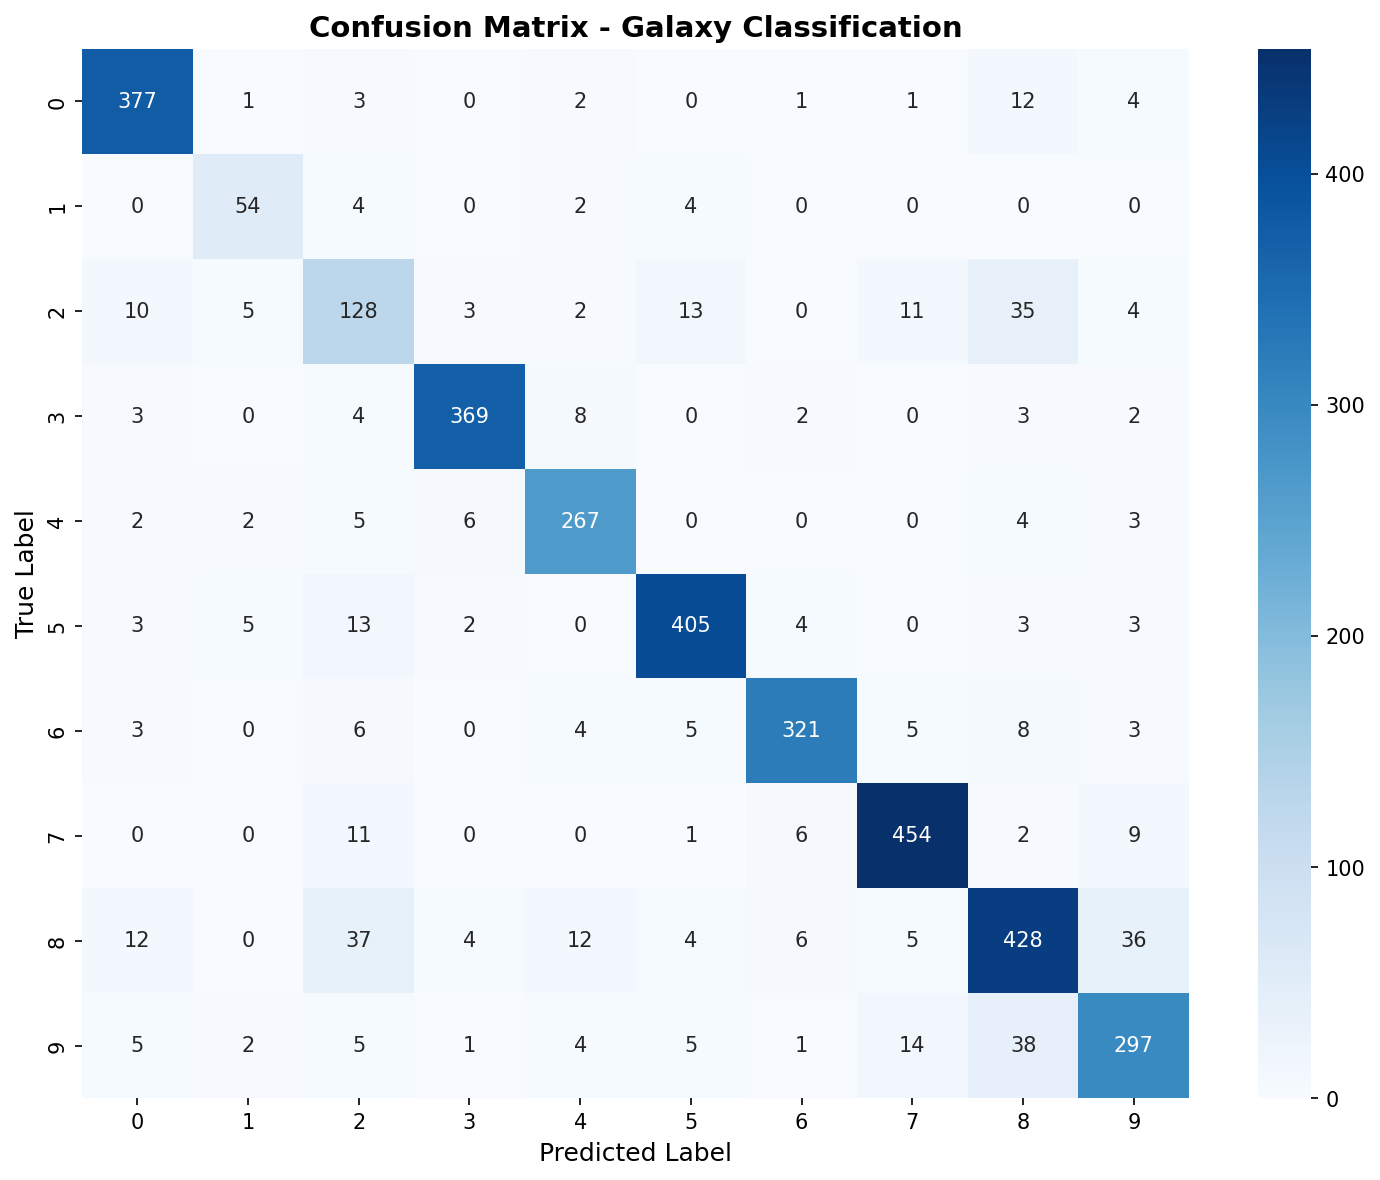
\includegraphics[width=0.75\linewidth]{confusion_matrix.png}
\caption{Confusion matrix on the validation set.}
\end{figure}

The confusion matrix shows strong diagonal dominance, indicating correct predictions for most classes.
Some confusion occurs between visually similar morphologies (e.g. irregular vs merging galaxies).

\begin{figure}[H]
\centering
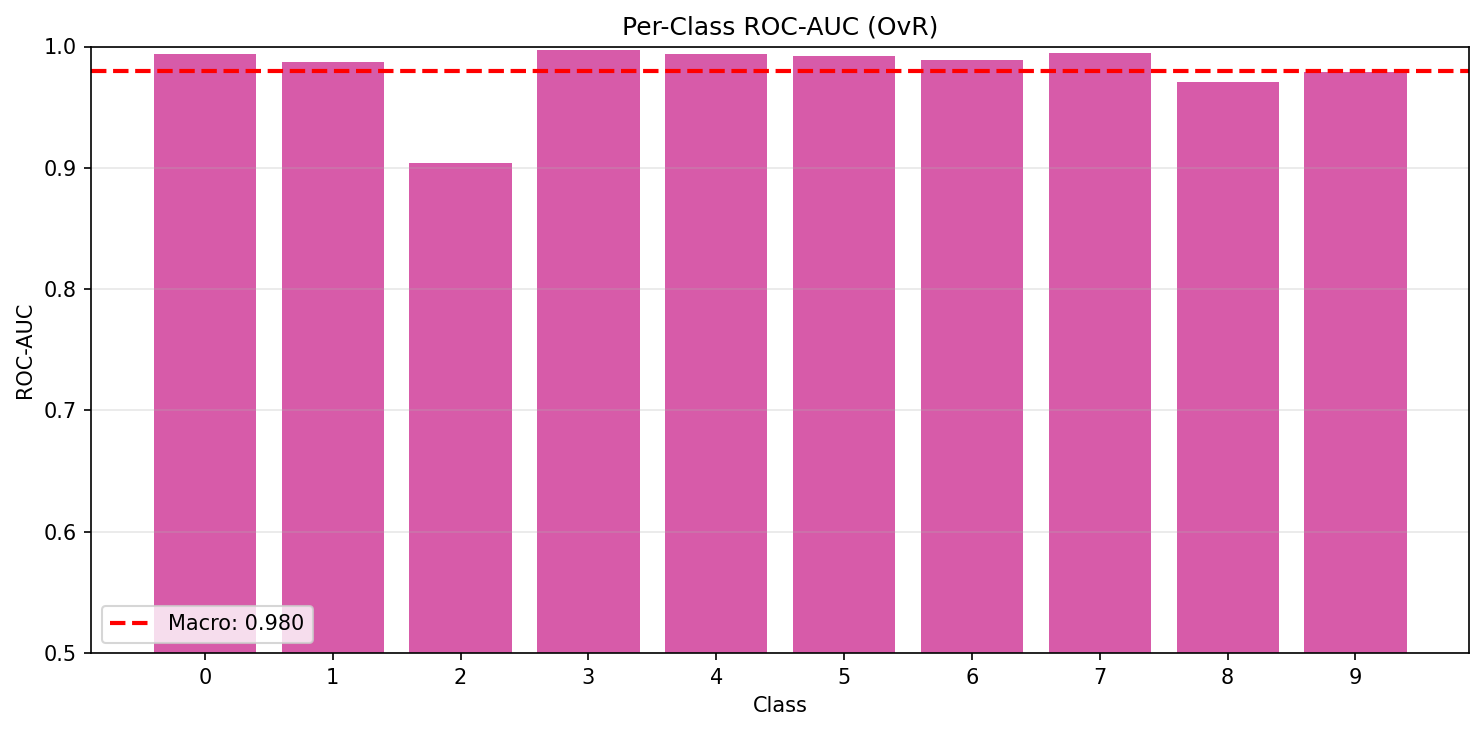
\includegraphics[width=0.75\linewidth]{roc_auc_scores.png}
\caption{Per-class ROC-AUC (one-vs-rest).}
\end{figure}

High ROC-AUC values demonstrate that the model separates galaxy classes with strong confidence.

\section{Robustness}

\begin{figure}[H]
\centering
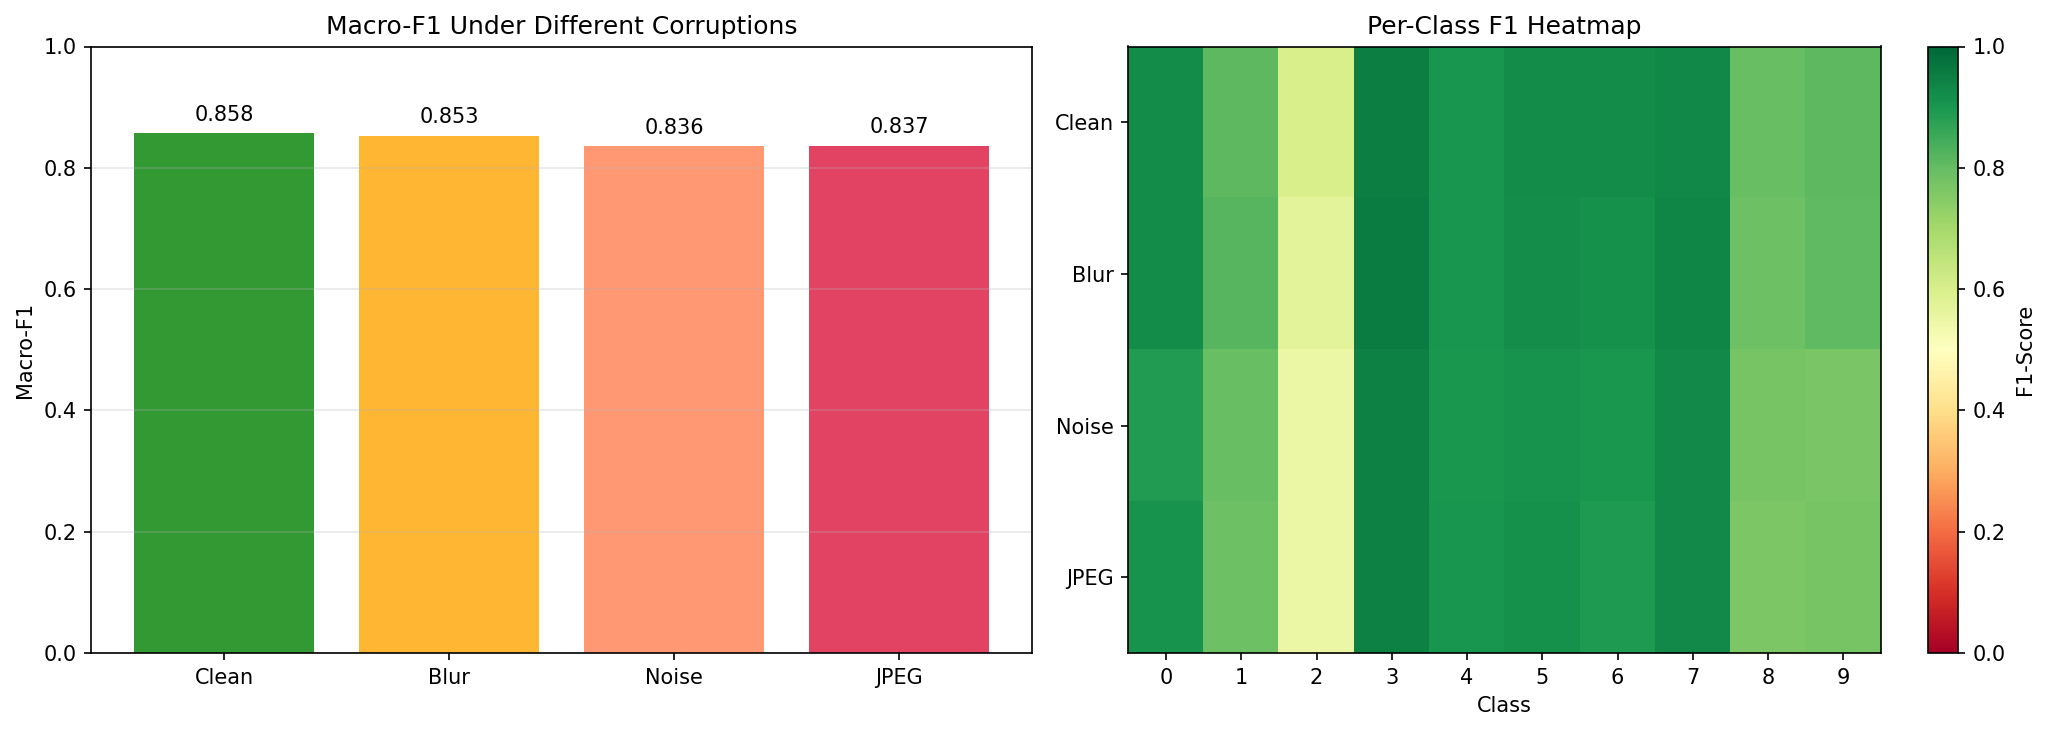
\includegraphics[width=0.75\linewidth]{robustness_comparison.png}
\caption{Macro-F1 under Gaussian noise, blur and JPEG compression.}
\end{figure}

Performance degrades most under blur, showing reliance on fine spatial structure such as spiral arms and bars.
JPEG compression has a smaller effect, indicating reasonable tolerance to storage artifacts.

\section{Conclusion}
We built a reproducible ConvNeXt-based system that classifies galaxy morphologies with strong balanced performance
(Macro-F1 = 0.86) and acceptable robustness to real-world distortions. The full pipeline and trained model are
publicly available.

\section*{Code and References}
\textbf{Project Repository (PS-1):}
\href{https://github.com/InfinityxR9/SpaceCode}{SpaceCode} (folder \texttt{ps1/})

\textbf{Dataset:}
\href{https://huggingface.co/datasets/Xanadu00/autotrain-data-galaxy_classification}{HuggingFace Galaxy Dataset}

\textbf{Team GitHub Profiles:}
\begin{itemize}
\item Aryan Sisodiya — \href{https://github.com/InfinityxR9}{InfinityxR9}
\item Daksh Rathi — \href{https://github.com/dakshrathi-india}{dakshrathi-india}
\item Priyanshu Baranwal — \href{https://github.com/priyanshubarnwal122-ai}{priyanshubarnwal122-ai}
\end{itemize}

\end{document}
